%!TEX root = tesis.tex

\newcommand{\w}{\emph{worker}\xspace}
\newcommand{\ws}{\emph{workers}\xspace}

\newcommand{\solveando}{\emph{solveando}\xspace}
\newcommand{\solvear}{\emph{solvear}\xspace}

\chapter{Un \ssolver paralelo y distribuido }
\label{ssolver-pardist}

El objetivo principal de todo sistema distribuido es que el mismo sea
\textbf{escalable}. Si bien la escalabilidad puede ser entendidad en
diferentes sentidos, nos interesa en particular que el sistema haga posible la
utilización de mayor cantida de \hard para resolver el problema (en nuestro
caso un problema \sat) y que esa utilización de mayor poder de cómputo reporte
ganancias en términos de tiempo (percibido) invertido en resolver un
determinado problema o bien en términos de empujar la frontera de lo
resoluble.

La escalabilidad como gran objetivo rector en el desarrollo de nuestra
herramienta introduce una serie de desafíos a saber:

La necesidad de que los nodos de trabajo (\ws) sean símetricos en
tanto que esto permite mayor dinamismo, y por lo tanto mejor utilización del
\hard disponible. La simetría entendida en su máxima expresión como la
posibilidad de que todas las unidades de procesamiento puedan realizar todas
las funciones necesarias provee la capacidad de distribuir la carga de trabajo
de la manera más conveniente en cada momento. Esto no podría ser logrado si
los nodos de trabajo tuvieran funciones específicas ya que se podría dar el
caso de tener nodos ociosos porque no hay trabajo pendiente de la clase de
trabajos que esos nodos saben realizar.

En nuestro caso particular esto se traduce en que los \ws deben poseer las
capacidades de: \solvear \todo{buscar una forma de decir esto que no sea
tan fea o en su defecto definir esto en la parte de preliminares} un
subproblema (consumir), dividir un subproblema en nuevos subproblemas
(producir) y almacenar, solicitar y transferir subproblemas (distribuir).

El triple rol de productor, consumidor y distribuidor asignado a los \ws hace
que la movilidad de tareas se transforme en un desafío en tanto que un \w
puede estar \solveando al mismo tiempo que otro \w le solicita una tarea
pendiente. Es evidente que en esta situación no es viable que el \w que está
esperando una tarea tenga que esperar a que el \w que tiene dicha tarea
termine de \solvear para que su pedido sea completado.

El objetivo global de escalabilidad también trae aparejado la necesidad de que
el almacenamiento de problemas pendientes de resolución se encuentre
distribuido. Esto se debe a un doble aspecto. Por un lado, la cantidad de
subproblemas producidos puede ser muy grande. Por lo tanto no es viable
requerir que la cantidad de espacio necesario para almacenar todas las tareas
pendientes de resolución se encuentre disponible en una ubicación. Menos aún
si pretendemos que nuestro sistema puede crecer en cantidad de \ws ya que este
crecimiento se traduce también en un crecimiento en la cantidad de productores
y por lo tanto en la cantidad de tareas producidas. Un segundo problema que
presentaría el almacenamiento centralizado es el de la contención. En este
aspecto, si pretendemos que el almacenamiento no se vuelva un cuello de
botella es vital distribuir de la mejor manera posible las tareas pendientes
de modo que cuando los \ws requieren nuevas tareas para resolver, los
múltiples pedidos no recaigan en un mismo equipo.

\newcommand{\ots}{\emph{off-the-shelf}\xspace}

Otro de los objetivos que perseguimos a la hora de diseñar nuestra herramienta
fue que la misma pudiera utilizar un \ssolver \ots. Esto nos permite
aprovechar los avances que se han obtenido en el área de \ssolving secuencial
en los últimos años (que han sido muchos) a la vez que nos permite, a futuro,
evolucionar a la par de los \ssolvers secuenciales de manera más simple. Esto
proporciona la posibilidad de que la herramienta no se vuelva obsoleta ante un
nuevo avance en \ssolving secuencial.

Generar una estrategia automática que provoque buenos resultados en la
ejecución de problemas diversos es sumamente difícil. Más aún, no tener la
posibilidad de modificar la estrategia adoptada durante una corrida que puede
ser sumamente larga puede tener resultados catastróficos. Esto nos motivó a
adoptar un enfoque en el que la maquinaria de cómputo distribuido no posee
inteligencia alguna y por el contrario provee una serie de opearciones
básicas. La operación del sistema por lo tanto se lleva a cabo desde un
\textbf{tablero de control} que permite al usuario manipular el sistema de
cómputo.


\begin{itemize}
	\item Escalable
	\item Uso de SAT Solver off-the-shelf
	\item Multiplataforma
	\item Tablero de control
\end{itemize}

\section{Arquitectura}
\missingfigure{Diagrama de arquitectura del solver}

\subsection{Lo del \cluster}

\subsection{El tablero de control}

\begin{figure}
	\begin{subfigure}[b]{0.5\textwidth}
		\centering
		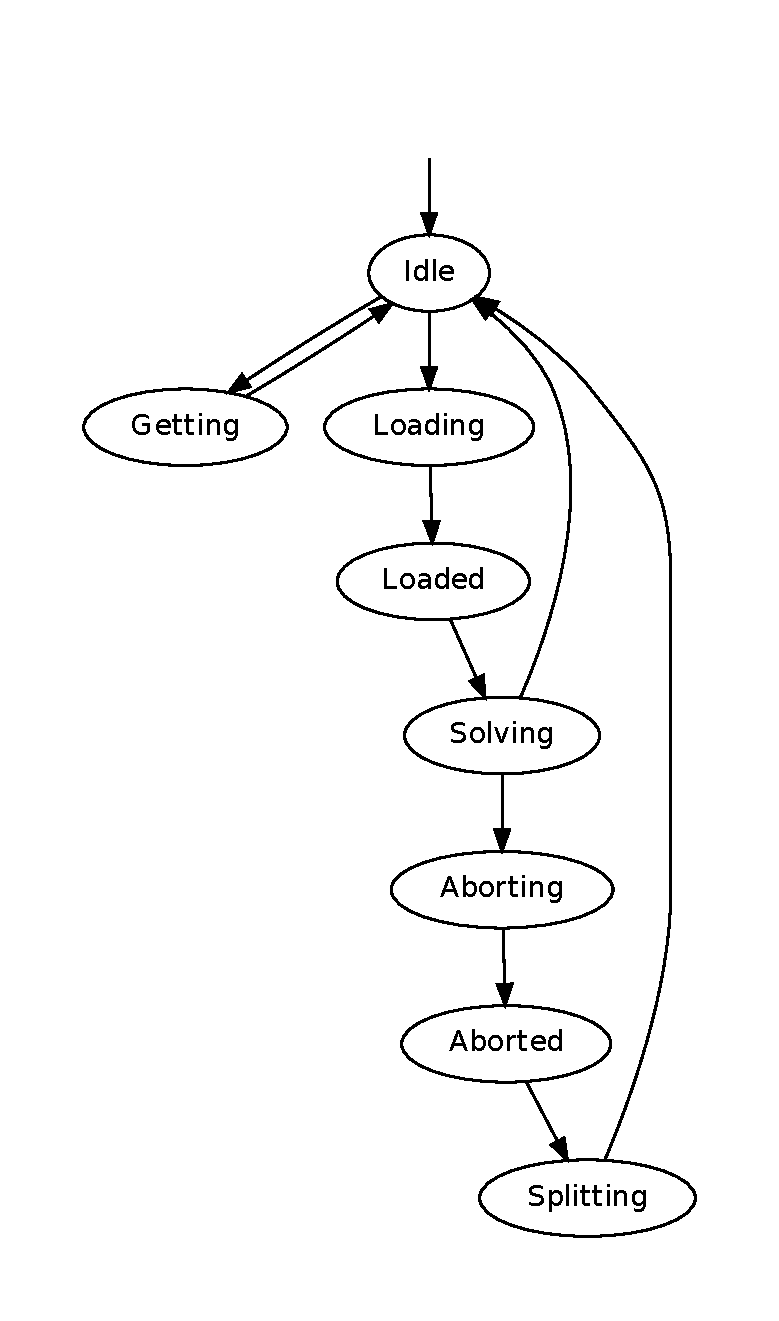
\includegraphics[scale=0.5]{graphs/workerstates}
		\caption{\emph{Workers}}
	\end{subfigure}
	\begin{subfigure}[b]{0.5\textwidth}
		\centering
		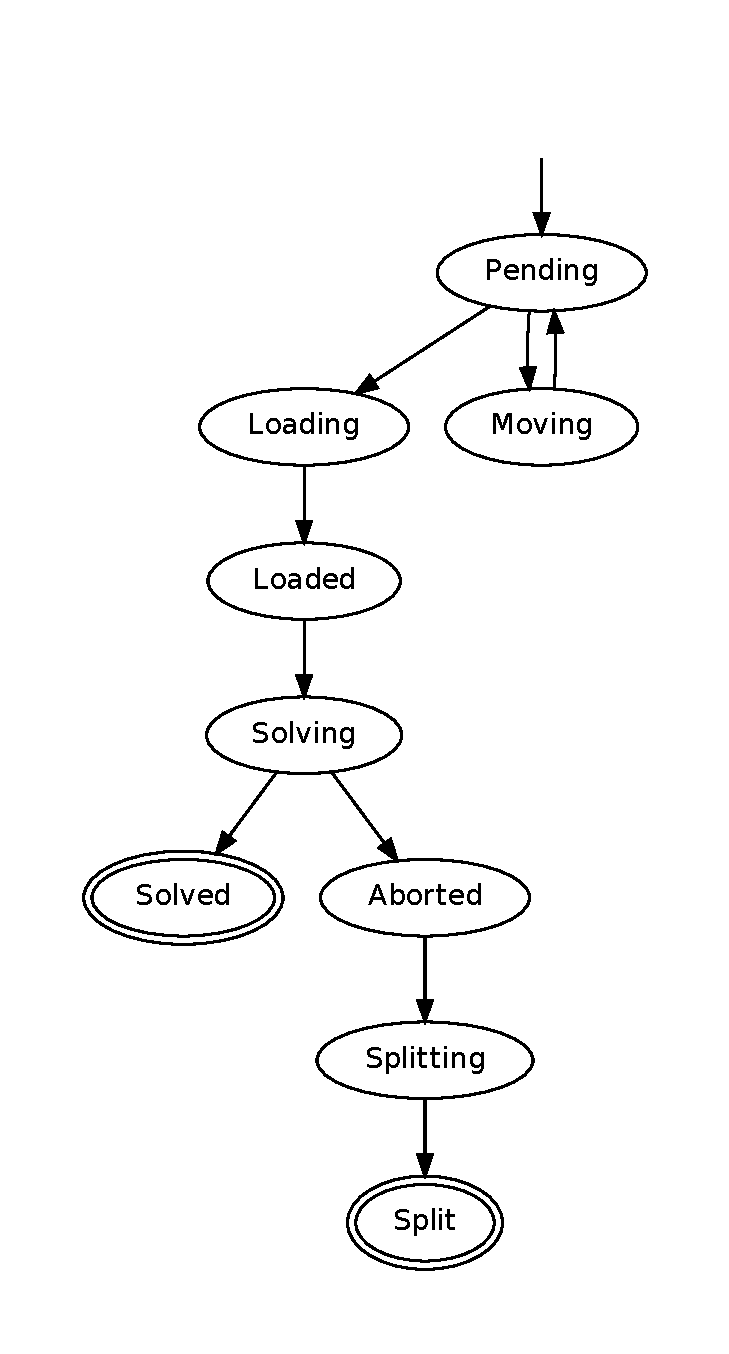
\includegraphics[scale=0.5]{graphs/taskstates}
		\caption{Tareas}
	\end{subfigure}
	\caption{Diagramas de estado en el tablero de control}
\end{figure}

\begin{small}
\begin{lstlisting}[language=Python,caption=Interfaz Strategy]
class Strategy(object):
	def register_globalstate(self, globalstate)
	def register_socket(self, commandsocket)
	def on_init(self, worker)
	def on_createroot(self, worker, task)
	def on_init_finished(self, nworkers)
	def on_getfile(self, worker, task)
	def on_file(self, worker, task)
	def on_load(self, worker, task)
	def on_unsat(self, worker, task)
	def on_sat(self, worker, task, modelstr)
	def on_abort(self, worker, task)
	def on_split_newtask(self, worker, newtask)
	def on_split_finished(self, worker, parenttask, nchildren)
	def on_shutdown(self)
\end{lstlisting}
\end{small}

\subsubsection{Nuestra estrategia}

\subsection{Decisiones que vale la pena seguir investigando}

\section{Resultados experimentales}